\documentclass[a4paper,fleqn,12pt]{article}

%%%%%%%%%%%%%%%%%%%%

\usepackage[utf8]{inputenc}

\usepackage[a4paper, total={6.5in, 9.5in}]{geometry} % sets content area width and height respectively

\usepackage{amsmath} %For both in-line and equation mode
\numberwithin{equation}{section} %Numbering of our equations per section
\usepackage{fancyhdr} %For our headers
\setlength{\headheight}{50pt}
\usepackage{fancyref}
\usepackage{graphicx} %Inserting images
\usepackage{setspace} %Spacing on the front page for crest and titles
\usepackage[]{fncychap} % Styles can be Sonny, Lenny, Glenn, Conny, Rejne, Bjarne and Bjornstrup
\usepackage[hyphens]{url} %Deals with hyphens in urls to make them clickable
\usepackage{xcolor} %Great if you want coloured text
\usepackage{tabularx}
\usepackage{appendix} %Take a wild guess slick
\usepackage{mwe} % Can't remeber what this does
\usepackage{float}
\usepackage{tikz} % for advanced diagrams
\usepackage{pgfgantt} % for the gantt chart

\usepackage[
backend=biber,
style=ieee,
sorting=none
]{biblatex}
\addbibresource{../common/bibliography.bib}

%KEEP THIS ONE LAST it's quite buggy, it allows you to click on links within the pdf and web links without changing the colour. The mouse cursor simply changes its icon to indicate to the user. Great tool - still awkward
\usepackage[hidelinks]{hyperref}

%This will tell the compiler to do the header style, page and spacing between the header and text
\fancyhf{}
\pagestyle{fancy}

%KEEP THIS ONE LAST it's quite buggy, it allows you to click on links within the pdf and web links without changing the colour. The mouse cursor simply changes its icon to indicate to the user. Great tool - still awkward
\usepackage[hidelinks]{hyperref}

\setlength{\parindent}{0mm}
\setlength{\parskip}{\medskipamount}
\renewcommand\baselinestretch{1.2}

\makeatletter
\newcommand{\@assignment}[0]{Assignment}
\newcommand{\assignment}[1]{\renewcommand{\@assignment}{#1}}
\newcommand{\@supervisor}[0]{}
\newcommand{\supervisor}[1]{\renewcommand{\@supervisor}{#1}}
\newcommand{\@yearofstudy}[0]{}
\newcommand{\yearofstudy}[1]{\renewcommand{\@yearofstudy}{#1}}
\makeatletter

\newtoggle{IsDissertation}

%%%%%%%%%%%%%%%%%%%%%%%%%%%%%%%%%%%%%%%%%%%%%%%%%%%%%%%%%%%%%%%%%%%%%%%%%%%%%%%
%% Project-specific configuration
%%%%%%%%%%%%%%%%%%%%%%%%%%%%%%%%%%%%%%%%%%%%%%%%%%%%%%%%%%%%%%%%%%%%%%%%%%%%%%%

\author{Zac Benattar}
\librarycardnumber{2112876}
\title{A Self-Practice App for Future Pilots}
\supervisor{Yulia Timofeeva}
\yearofstudy{3\textsuperscript{rd}}

%%%%%%%%%%%%%%%%%%%%%%%%%%%%%%%%%%%%%%%%%%%%%%%%%%%%%%%%%%%%%%%%%%%%%%%%%%%%%%%


\setcounter{secnumdepth}{0} % disables section numbering

\assignment{Project specification}

%%%%%%%%%%%%%%%%%%%%

\pagestyle{plain}
\renewcommand{\headrulewidth}{0.0pt}

% sets up header with name, project and footer with page num
\makeatletter
\fancypagestyle{plain}{
	\fancyhf{}
	\fancyhead[R]{\textit{\@title} - \textit{\@assignment}}
    \fancyhead[L]{\textit{\@author}}
    \fancyfoot[C]{\thepage}
}
\makeatother

%%%%%%%%%%%%%%%%%%%%

\begin{document}

\pagestyle{plain}

\chapter{Introduction}
\label{ch:introduction}

Write around four paragraphs establishing the context and motivating your project.

Radiotelephony (R/T) is the language of flight crew and air traffic control (ATC) in radio communication. As a specifically structured subset of spoken English, it provides a global standard for aircraft communication when supplemented with Aviation English. Though many countries with high aircraft traffic have their own versions, they all closely follow the international standard as defined by the International Civil Aviation Organisation (ICAO) in Document 9432 \cite{Doc9432}. In the UK, prospective pilots and flight crew must pass both a R/T theory and practical exam as part of their licensing process. A common process for practising for the practical exam involves learning the CAP413 document which defines standard R/T in UK airspace \cite{CAP413}, then organising mock tests with an examiner. Organising mock tests is expensive and time consuming, hence practice software that imitates exam scenarios are frequently used as part of a student's practice routine. The main issue with existing practice software is the lack of speech input capability. Requiring users to enter their radio messages in text form somewhat limits the quality of the practice. It would thus be useful for trainee pilots to have access to a solo practice system which provides mock test like conditions without the need for an examiner to play the part of ATC, while supporting speech input.

\section{Related work}

Although limited by a lack of voice input support, two high quality and popular R/T practice applications are currently available online.

Readability5 presents a simple interface which mimics the resources a student would have in the exam \cite{Readability5}, that being a radio, transponder, map, and kneeboard (a notepad often attached to a pilot's upper thigh). In each module the user is walked through a scenario in which, mimicking the actual exam, they must select the correct frequencies and modes on both the radio and transponder and transmit radio calls. Five modules which teach different aspects of R/T can be purchased, however the route used in each module is fixed, so once a module has been completed once, the next practice will be on the exact same route. Voice input is technically supported, but all speech is considered correct, so users can simply press the transmit button without saying anything and progress to the next state in the scenario.

Wilco Radio is a feature rich training system which provides many practice modes including mock tests \cite{Wilco-Radio}. Its interface shows much more information than that of Readability5, much of it being unnecessary for the exam. It also does not support the managing of radio and transponder frequencies and modes, which are part of the skills required to pass the R/T exam. Its fundamental flaw is the form of input it supports - users select from a set of predefined options given by the system to respond to each radio message. Despite this, it does provide extensive feedback on radio calls, and shows the user's progress metrics including the number of procedures practised, and the user's accuracy rate.
% Add images

\section{Objectives}

RT-Trainer, as the system has been named, aims to recreate many of the 

\begin{enumerate}
    \item Generation of random scenarios with suitable random locations, events, and radio messages for R/T exam practice.
    \item Allow users to practice the scenarios by typing or speaking each radio call when prompted.
    \item Support for up-to-date modern browsers (at least Chrome, Safari, Firefox and Edge).
    \item Feedback on the accuracy of a user's radio calls.
    \item User statistics and progress tracking.
    \item Allow sections of scenario to be practised separately.
    \item Provide multiple levels of support while practising.
    \item Allow sharing of scenarios between users.
\end{enumerate}

Note that objective 7 was not met so is not included in the implementation section. Objective 8 was completed before 7 due to the design of the system providing the means for users to share scenarios without any extra code.

\section{Background}
\label{sec:background}
The use of automatic speech recognition has been trialled in an aviation communication context by various researchers over the last decade, but so far these efforts have been related to reducing workload or improving reliability of ATC. Projects such as STARFiSH (Safety and Artificial Intelligence Speech Recognition) have been funded by governments as a modernisation program for ATC with some success \cite{STARFiSH}. The main challenge with such efforts is found in the safety aspect. This project however, is related to the other party in the radio communication, the pilot.

% https://www.malorca-project.de/wp/wp-content/uploads/Ohneiser_Oliver_1474.pdf
% Paper on using a similar system to provide suggestions/optional decisions for ATC based on their radio calls and a model of the status of each flight they are managing
%  Although the usage of data link in ATC is discussed at least since the 90s, voice communication will definitely remain a pillar of air traffic control. The Strategic Research & Innovation Agenda (SRIA) of ACARE (ACARE, 2012) or Flightpath 2050 (European Commission, 2011) do not expect a fully automated ATM (Air Traffic Management) system in the next decades.

Pilots' R/T skills have been identified as a common weak spot by many aviation agencies \cite{flight-safety-failure-to-communicate}. A study by Istanbul Rumeli University recently found that 7 of the 20 deadliest aircraft collisions were caused by communication errors \cite{communication-in-accidents}. Famously, the deadliest aviation accident in history, the Tenerife airport disaster, was caused by miscommunication \cite{tenerife-accident-description}. The pilot of KLM flight 4805 mistaking an instruction from ATC referring to takeoff without giving permission, as permission to take off \cite{tenerife-accident-description}, resulting in an impact with Pan Am flight 1736 taxiing down the same runway. Significant changes to communication procedures and the grammar of R/T were implemented after the disaster \cite{CAP413-ed15-ch2-p6}, and changes continue to be implemented following other incidents.

Given the fundamental nature of communication in aviation and its resulting high safety levels, correctness, brevity and confidence are important for radio calls. Pilots must be correct in their calls to avoid dangerous situations. Communications should be short as radio communications support only one speaker at a time. Confidence ensures that calls are made at the right time, and are not the main focus of the pilot, which should be controlling the aircraft. The project's client, a R/T instructor based at Wellesbourne airfield, has encountered many pilots, both student and commercially operating, with poor R/T skills in the air.

The Coronavirus pandemic has increased the need for pilot refresher training, with the European Union Aviation Safety Agency (EASA) releasing guidelines on extra training for pilots and ground staff who are coming back from an extended break from work \cite{EASA-Training-Post-Covid}. Given the nature of the flight profession, pilots may not be able to attend regular in-person training if they are travelling. A system that offers online solo practice with no need for arranging an instructor could form part of a pilot’s continued skills practice.

\subsection{Existing Software}
Although limited by a lack of voice input support, two high quality and popular R/T practice applications are available online. Neither are open source, hence this project will involve developing many of the features found in these systems, with the addition of voice input.

Readability5 presents a simple interface which mimics the resources a student would have in the exam \cite{Readability5}, that being a radio, transponder, map, and kneeboard (a notepad often attached to a pilot's upper thigh). In each module the user is walked through a scenario in which, mimicking the actual exam, they must select the correct frequencies and modes on both the radio and transponder and transmit radio calls. Five modules which teach different aspects of R/T can be purchased, however the route used in each module is fixed, so once a module has been completed once, the next practice will be on the exact same route. Voice input is technically supported, but all speech is considered correct, so users can simply press the transmit button without saying anything and progress to the next state in the scenario.

Wilco Radio is a feature rich training system which provides many practice modes including mock tests \cite{Wilco-Radio}. Its interface shows much more information than that of Readability5, much of it being unnecessary for the exam. It also does not support the managing of radio and transponder frequencies and modes, which are part of the skills required to pass the R/T exam. Its fundamental flaw is the form of input it supports - users select from a set of predefined options given by the system to respond to each radio message. Despite this, it does provide extensive feedback on radio calls, and shows the user's progress metrics including the number of procedures practised, and the user's accuracy rate.

\begin{center}
    \begin{tabular}{ | c | m{24em} | c | c | }
        \hline
        \bf{Num} & \bf{Objective} & \bf{Priority} & \bf{Prerequisites} \\
        \hline
        1 & The system will provide scenarios suitable for RT exam practice & High & None \\
        \hline
        2 & The system will generate random flight scenarios with suitable random locations, events and radio messages & High & 1 \\
        \hline
        3 & The system will allow students to respond to scenarios and provide feedback on responses & High & 1 \\
        \hline
        4 & The system will be web based and function correctly on modern browsers & High & None \\
        \hline
        5 & The system will allow voice responses via a speech to text system & High & 3 \\
        \hline
        6 & The system will allow students to view progress and statistics of their learning so that the student can see areas to focus on & Medium & 1, 3 \\
        \hline
        7 & The system will allow students to select a support level ranging from fully guided scenarios to no guidance exam like conditions & Medium & 1, 3 \\
        \hline
        8 & The system will allow students to select smaller parts of scenarios to practice specifically as to not waste time on sections they are already confident with & Medium & 1, 3 \\
        \hline
        9 & The system will allow students to save for later or share specific scenarios with other students by providing a seed for the random number generator used in scenario generation & Low & 2, 3 \\
        \hline
        10 & The system will have sub 5 second latency when responding to a user's voice input & Low & 5 \\
        \hline
    \end{tabular}
\end{center}
\subsection{Methodology}
This project lends itself to being suitable for an agile development methodology, given that it is small with a single inexperienced developer, requirements and time constraints may change, and having frequent builds with new progress ensures that a functioning product will exist by the end. Sprints will range from 1-3 weeks long depending on the difficulty of the task being worked on in that sprint, and the time available to work on the project during the sprint. 

To ensure that the software meets the requirements set out by the customer, the objectives settled on have been based on a similar set of requests from the customer, and communication with the customer will continue through the project. Various builds may be provided to get feedback that can be implemented in the next sprint.

Supervisor meetings will occur frequently when progress has been made or extended discussion of ideas is required, but will be arranged week to week to avoid unnecessary meetings and to balance availability of myself and my supervisor.

All project code and documents will be stored in a GitHub repository with CI\textbackslash CD configured in GitHub Actions to ensure the latest production version compiles and is always hosted via GitHub Pages. Online hosted version control ensures that access to the codebase and documents is simple and always available, and that mistakes can be reverted if needed. CI\textbackslash CD ensures that a testable version of the project is available at all times so feedback can be gained more often and on a recent version and no extra effort will be required to create a functioning prototype for the presentation.

\subsection{Timetable}
Taking into account deadlines for both this project and for the coursework of other modules, an initial timetable includes all essential parts of the system in term 1, with the most important features implemented by the due date of the progress report. Additional features will follow during the winter holidays and term 2. Task dependencies are mostly linear with each task requiring the previous one to be completed, or only makes sense to be completed after the previous one because the tasks are planned to be undertaken in order of importance. Each task will include a substantial amount of time spent researching how to perform it, such as identifying suitable technologies, APIs or data required to implement a feature. It is expected that this timetable will be accurate only in the short term, given that projects of this scale are very likely to encounter delays caused by unforeseen issues, hence an up to date version of the timetable will be maintained. Some possible delay causing events are clashes with the completing of coursework from other modules, so a longer period of time has been allocated to tasks which should be performed during these periods, which also gives time for breaks from the project.

% Gantt image
\begin{figure}[H]
    \centering
	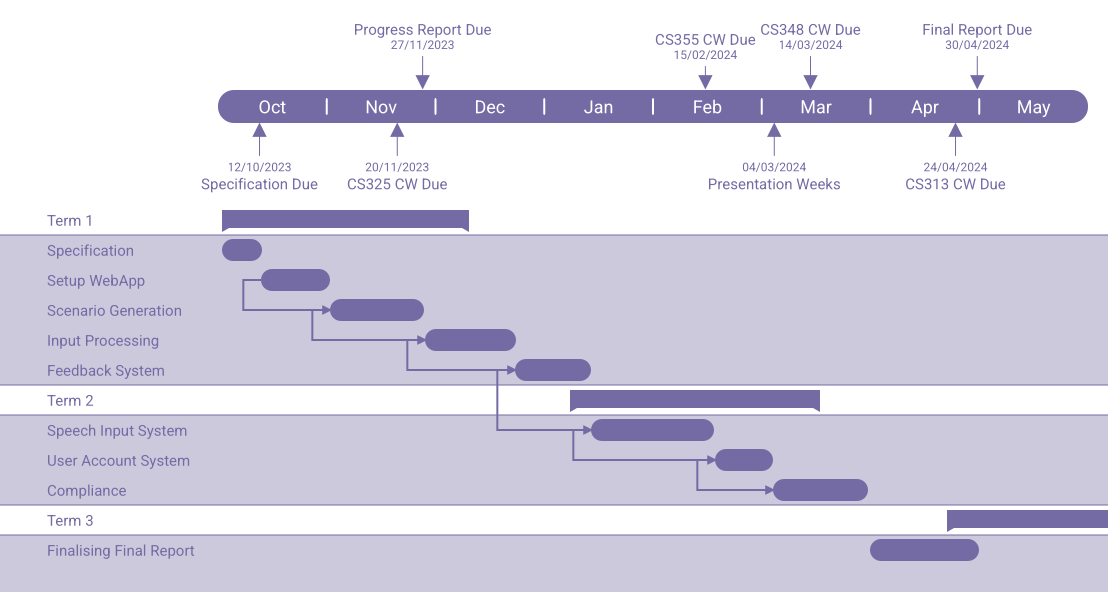
\includegraphics[scale = 0.42]{../document-resources/images/initial-gantt.png}
    \label{initialgantt}
    \caption{Proposed project timeline}
\end{figure}

\subsection{Risk Assessment}
The risks involved in this project are primarily related to the people and technologies required to build it.
The technology risks include access to the APIs that will be relied upon to obtain data which I cannot feasibly obtain myself within the scope of the project.
At any time the APIs could be changed or removed, which would require a change in the project scope, but can be somewhat mitigated by keeping features modular, so that they can be removed or replaced with minimal impact on the rest of the system.
The Google Maps API is free for \$200 worth of transactions per month, which should be sufficient for the project. However, it is possible that this limit be reached, which would require reconsidering the use of the API, but other similar APIs exist such as the Bing Maps API which offers limited educational usage.

Given that implementing even pre-trained machine learning models can be difficult, the speech to text conversion may need to be done by an external API if time constraints require it. Various such APIs exist with free tiers of access suitable for the project.

\subsection{Resources \& Technologies}
\begin{itemize}
    \item GitHub Repositories, Actions and Pages. Using a version control system reduces development issues and improves code availability.
    \item Languages: Javascript, HTML, CSS. Performance will not be a major requirement as the expected user count is low for the system, hence Javascript is suitable as it fields countless libraries and provides a good developer experience.
    \item Libraries: Whisper for Speech to Text conversion, Svelte Web Framework \& SvelteKit for simplifying web app development.
    \item APIs: Google Maps API for aerial map data, Google Speech API (if own implementation proves infeasible).
    \item Customer
    \item Documents: CAP413 RT manual.
\end{itemize}

\subsection{Legal, Social, Ethical, Professional Issues and Concerns}
Given that the target users of the system will mainly be trainee pilots, it is paramount that the information taught by the system follows the guidelines set by the UK Civil Aviation Agency (CAA), given that incorrect or insufficient teaching has shown itself to be a factor in the causes of multiple aircraft incidents in the last two decades. If the software is to be used for training, care must be taken to insure that it reflects correct teaching of radio communications as set out in the CAP 413: Radiotelephony Manual \cite{CAP413}. This could be resolved by working with trained flight instructors and examiners to validate the system's information, and the inclusion of a notice to all users that the software should only be used alongside lessons from a qualified instructor.

\printbibliography

\end{document}
